\documentclass[a4paper, 12pt]{article}

% packages
\usepackage{fancyhdr}
\usepackage{setspace}
\usepackage{parskip}
\usepackage[hidelinks]{hyperref}
\usepackage{xfrac}
\usepackage[margin=1.2in]{geometry}


\begin{document}

\begin{titlepage}

% defines new rule for horizoontal lines & thickness
 \newcommand{\HRule}{\rule{\linewidth}{0.5mm}}
 
 \center % center everything
 
 \textsc{\LARGE Loughborough University}\\[1.5cm]
 
 \textsc{\Large COP507}\\[0.5cm]
 
 \textsc{\large Computer Vision \& Embedded Systems}\\[0.5cm]
 
\HRule\\[0.4cm]

 {\huge Report on Vehicle Make and Model Recognition System}\\[0.4cm]

\HRule\\[1.5cm]

\begin{minipage}{0.4\textwidth}
 \begin{center}
   \large
   \textit{Author}: \textsc{Ekow Mensah (B717426)}
 \end{center}
 \end{minipage}

\vfill\vfill


\includegraphics[width=0.7\textwidth]{logo.png}\\[1cm]

\vfill\vfill\vfill
{\large\today}

 
\end{titlepage}
 
 \newpage
 
 \tableofcontents{}
 
 \newpage
 %---------------- introduction ------------ %
 
 \section{Introduction}
 \onehalfspacing
 Make and Model Recognition (VMMR) has been a subject area of interest within computer vision both in industry and academia. The importance of the ability to recognise a variety of vehicles spans across different disciplines and applications such as driver assistance, traffic monitoring, law enforcement and surveillance. As stated by Dehghan et al (2017), this categorisation task has been a problem for classical computing however, a result of great advances in artificial intelligence, this task has been made possible with accuracy rates above 90 percent. The task given was to design and implement a VMMR system with the capability to recognise the make and model of a vehicle based on only the front view (that is, headlights, grill and bumper). Based on the image of a vehicle fed as input, the output of the system should be the make and model of the vehicle. This report explains a practical use of the VMMR system that was implemented, furthermore, it explains the design of the system and any performance restrictions or performance enhancements that will be expected should the system implemented in hardware.
\parskip 0.2in 

There some basic processes that are essential for any computer vision application. These include pre-processing the acquired images, feature detection and feature extraction. Pre-processing involves making the image data conducive for feature extraction. Some of these processes includes noise reduction, morphological operations, colour correction and image re-sampling. Feature extraction is the process by which key points are obtained from the image. These key points consist of blobs, edges and corners.
 
 \newpage
 
 %--------------- Section 2: Preprocessing Tasks ------------------ % 
 \section{Preprocessing Tasks}
 This section discusses the pre-processing tasks that are required to implement the Vehicle Make and Model System in practical scenarios.
 
 \subsection{CCTV camera located at the side of a motor way}
 As a consequence of this system being implemented outdoors, there are certain factors that cannot be controlled prior to the CCTV footage being taken. These factors include illumination, motion blur, problems with focus and the camera being placed at an angle  which affects processing of the image. The following subsections explain solutions to these problems found when processing the images taken by the camera. 
 
 \subsubsection{Skewing \& Rotation}
Considering the camera is at the side of the motor way, one thing to consider is that the angle at which the camera is placed. Therefore, before performing any feature detection or extraction, the images taken from that camera must be set to the right orientation. This could be done by skewing the image or rotating the image as this will set the image to the right orientation. Traditional mathematical algorithms and formulas exist which can be used to correct the angle of rotation or the degree of skewing required. Considering that since an image can be represented as a matrix of pixel values, affine transformation matrices could be applied to the image to correct the problem (Gonzales \& Woods, 2008).
\parskip 0.2in 

Before these algorithms can be applied to the images, it must be detected whether there is a need to apply skew correction to the images captured. Patel et al. (2015) discuss an approach for skew angle detection and correction based on the radon transform. The radon transform was used because of its accuracy and low computational cost. The radon function calculates projections of the image matrix in particular directions (Patel et al, 2015). For an image matrix \textit{f(x,y)} a projection is considered as a collection of line integrals. The line integrals are calculated from various sources along beams, lateral paths, in a specific direction. The skew detection algorithm proposed by Patel et al (2015) is as follows. First of all, the input image is binarised and morphological filling operations are applied. After that, edges are detected using the canny edge detector. This process is used for locating relevant transitions within the image. The radon transform is then applied on the output of the edges detected. Next, a maximum value is searched for within the radon transform coefficients. After that, a skew angle is found from the maximum intensity value that was found from the radon coefficients. The image is then rotated with the skew angle. 

\subsubsection{ Brightness \& Colour Correction }
Another factor to consider is the lighting conditions. The reason being that, in the day time, pictures taken may or may not have the appropriate lighting. In the night time, the images taken may be very dark. Therefore, in order to make the images conducive for training, the images will need to be made brighter. A remedy to this problem could be applying a brightness adjustment algorithm. According to Szeliski (2010), this can be done by multiplying or adding the image by the constant. 

\begin{center}
 $g(x) = \alpha f(x) + \beta$ 	(Szeliski, 2010)
\end{center}

Where $\alpha$ and $\beta$ are parameters which influence the contrast and brightness of the image and where $\alpha$ is greater than zero. 

Alternatively, colour balancing and correction algorithms can be used to improve the illumination and contrast of the image. Weng et al (2004) introduce a novel approach of improving white balance in still images. This algorithm is needed especially for images taken at night because, depending on the colour temperature of the street light. The image will appear reddish if the colour temperature of the light source is low, conversely, the image will appear blue if the colour temperature of the light source is high (Weng et al, 2014). Therefore, improving the white balance will make the image appear as though it was captured under canonical lighting. 
\parskip 0.2in

The proposed solution works in two stages that is, white point detection and white point adjustment. utilises a dynamic threshold for identifying white points within the image. The process begins by converting the image from the $RGB$ colour space to the  $YC_{b}C_{r}$. Depending on the colour characteristics, a near white region composed of several candidate reference white points is chosen. The candidate points are chosen by computing the mean values of $C_{b}$ and $C_{r}$ (Weng et al, 2014). The white reference points are then selected depending on the brightness values  of candidate white points (top 10 percent) near the white region. After the white reference points have been chosen, the Von Kries model is used to fine-tune the image. This model is used to scale each invidivual $R, G$ and $B$ channel separately. Channel gains are obtained from the average values of reference white points. Luminance is maintained throughout the image at the same intensity by using the maximum luminance value to compute channel gains. Each pixel value is adjusted by multiplying each pixel with teh computed gain (Weng et al, 2014). 

\subsubsection{ Motion blur removal}

Motion blur is a phenomenon which occurs when there are inconsistencies between the speed of the moving object and the rate at which the camera captures frames. The problem with motion blur is that, it attenuates the image signal. Removing the motion blur from the image involves two processes. Firstly, estimating the amount by which the image has been blurred and thereafter, recovering a more realistic image using  deconvolution (point-wise division in the frequency domain). Cho (2010) proposes a method of deconvolution referred to as iterative distributed reweighting (IDR) for removing motion blur. This method enhances the visual quality of reconstructed images as compared with traditional deconvolution algorithms used for removing motion blur.
\parskip 0.2in 

Cho (2010) suggests the estimation of the blur kernel by examining edges within the blurred image. The edges within the blurred image encode estimations of the blur kernel from which the blur can be removed using the inverse radon transform. Using the edge information in this case will yield desirable results because, the object of interest is a man made object and man made objects consist of many edges. As a result of the loss of high frequency information, prior information concerning natural images is used to fill out the missing information. This is done using content aware image priors rather than sparse priors because, content aware prior adjusts its features to local textures and hence, it increases the quality of textures within the reconstructed images (Cho, 2010). After this has been completed, a maximum a posteriori (MAP) estimator is used to restore the image using piecewise smooth features, however, since the MAP does not always accurately reconstruct rich textures, IDR is used to improve the depiction of rich textures. 

\subsubsection{Shake Removal}
In the process of capturing images, the camera could be susceptible to shaking especially in windy conditions. This is a problem because, the camera shaking causes non-uniform blurring cannot be handled effectively by blind convolution algorithms (Hirsch et al, 2011). They suggest a fast single image  blind deconvolution algorithm which is a combination of both constraints of Projective Motion Path Blur (PMPB) models and the effectiveness of the Efficient Filter Flow (EFF) framework. In order to recover a sharper version of the image, EFF estimates a non-static blur as the total of various blur patches. The blur kernels are created using homographies. The homographies are then applied to a grid of pixels. This makes it possible to generate possible camera shakes via a combination of various homographies of a point grid (Hirsch et al, 2011). Different views of a point grid are created by using a homography. This splits the views into local blur kernels which are constrained to only linear combinations. 

\parskip 0.2in
Given a blurred image, an unknown sharp  image can be reconstructed in two steps: (1) blur estimation for non-stationary PSFs and (2) sharp image recovery through a non-blind deconvolution process suited to non-static blurs. The first step of the algorithm aims at retrieve the motion which the camera undertook during exposure provided only the blurry image. This involves a prediction phase, to lower the blur effect and improve image quality bilateral filtering, a blur parameter estimation phase to identify camera motion features which correctly describe the blurred image from the previous step and a latent image estimation using non-blind deconvolution (Hirsch et al, 2011). Blur parameters are approximated by finding the most appropriate non-static blur which converts the  immediate image estimate into the recorded blurry image. Sharp image updates are applied repeatedly during the blur estimation phase. After the blur parameters have been approximated and set, the final sharp image is reconstructed by replacing the image prior of the sharp image update phase with a more natural image prior which is formed on sparsity of gradient images (Hirsch et al, 2011). stationary non-blind deconvolution is then used in the non-stationary case to retrieve the sharp image. 

\newpage
\subsection{Dedicated camera installed at entrance to indoor car park}

Similar to the CCTV camera located at the side of the road, this system is affected by certain factors which may affect the quality of the images captured by the camera although not as much as an outdoor system. For instance, location at which the camera is placed can be controlled and hence it is placed at the best location possible (that is, the entrance of the car park).

\subsubsection{Noise Removal}

Noisy images might be a problem that may be experienced with images taken in camera located in the indoor car park. This noise occurs as a result of arbitrary variances in image intensities which appear as grains in the image (Kaur, 2015) . Noise is undesirable because it distorts the image signal and reduces the image quality. Kaur (2015) explains some primary sources of noise in images. These include poor light levels and the temperature of the sensor, electromagnetic transmission of the image data, effects of the environment on the image sensor, introduction of noise by the mechanism capturing image data in digital format, dust particles present on scanner screen. Noise can be removed using various techniques however the technique explained in this report is filtering (linear and non-linear). 
\parskip 0.2in

Linear filters eliminate certain types of noise by convolving the noisy image with a kernel which serves as a low pass filter (Kaur, 2015). Non-linear filtering on the other hand, produces an output which is not a linear function of its input. Using a gaussian filter to remove noise will be a viable solution however, the problem with using a gaussian filter is that, although it removes the noise, it also blurs the sharp edges and destroys useful details within the image. Therefore, using non-linear filtering is a much better solution because, non-linear filters preserve the image details in the image. For this scenario the preferred filtering technique is using a median filter. Median filters work by using a sliding window principle over the image matrix and replaces pixel values with the median value of neighbouring values. Initially, all pixels values are arranged from neighbourhood to numerical order. The pixel being considered the middle pixel value is then replaced (Kaur, 2015). Moreover, the median filter although simple, is very powerful and easy to implement. 

\subsubsection{Improving low resolution images}

Assuming that the camera being used captures low resolution images, it is essential that the quality of the images are improved before being passed to the next phase. Similar to noise removal, there are various methods of improving the image quality. however in this scenario, Freeman et al (2002) present a method of improving image quality using super-resolution. Their approach involves using interpolation algorithms to generate tenable high frequency details in zoomed images from a database of training images. This can be used to enhance the quality of low resolution images. 
\parskip 0.2in

The algorithm works by upscaling the images using cubic spline interpolation and downscaling using convolution with a [0.25 0.5 0.25] filter and subsampling
when indicies obtained are even. The super-resolution algorithm then anticipates the next octave up that is, the lost frequencies from the image using cubic interpolation. The result the algorithm produces is total of the inputs and high frequency estimates. The high frequencies are estimated for $M$ x $N$ patches in raster scan order (Freeman et al, 2002). The algorithm functions under the presumption that, the association between high and low frequency patches is not affected by contrast, hence each patch is normalised by the median absolute value of the low frequency patches in the colour channels. These frequency patches are then merged together to form a vector that is used to search for matches in the training set. The matching is accomplished by locating the closest neighbour. When matches are located, the contrast normalisation is undone on the matching high frequency patch and that patch is added to the output image.  


\subsubsection{ Removal of Barrelling Effect}

According to Gribbon et al (2003), The barrelling effect also known as barrel distortion is a phenomenon which happens when the magnification of the lens reduces with axial distance and hence, resulting in rapid movement of image points in the direction of the image centre. Gribbon et al (2003) define the barrel distortion model as: 
\begin{center}
 $r_{u} = r_{d}(I+kr^{2}_{d})$. (Gribbon et al, 2003).
\end{center}

Where $r_{d}$ and $r_{u}$  represent the lengths from the centre of the distorted and undistorted images. The barrel distortion algorithm works by calculating the position of the pixel within the barrelled image. After computation, the resulting coordinates are seldom integers. This problem is solved using bilinear interpolation. The barrel model presents the pixel positions (coordinates) of the undistorted image as a function of the pixel positions of the distorted image, however Gribbon et al (2003) argue that, this representation is not suitable for correcting the distortion in real time, because, the output of the undistorted pixels must be in raster scan order. Therefore, the coordinates of the image without barrelling must be used to decide the pixel to display in the distorted image. Hence the first equation is rewritten in terms of a radial independent magnification with a magnification factor $M$. This can be seen below: 

\begin{center}
$M = \frac{1}{1+kM^2r^{2}_{d}}$ (Gribbon et al, 2003)
\end{center}

The equation above is used to solve for $M$ repetitively until $M$ moves or converges towards the required precision (Gribbon et al, 2003). Bilinear interpolation was implemented by shortening the computed coordinates by rejecting the fractional element. This leads to rounding errors in the pixel location and hence produces artefacts. The algorithm derives the pixel values by computing the weighted sum of pixel values of four nearest neighbours surrounding the computed coordinates (Gribbon et al, 2003). 


\subsubsection{Contrast Stretching}
Images captured from the entrance of the car park may contain night glare caused by the light emerging out of the headlights of the car. This glare effect is undesirable because, it can result in an image having poor contrast. A solution to this problem is to use contrast stretching. Contrast stretching aims to enhance the contrast by expanding the range of intensity values within the image across the range of pixels allowed by the input image (Fisher et al, 2003). To perform contrast stretching first, the lower and upper pixel limits which determine the pixel range for the normalisation process must be defined. The image is then scanned to identify the highest and lowest pixel values within the image. Suppose that the lower and upper pixel limits are $i$ and $j$ respectively and the highest and lowest pixel values are $k$ and $l$ respectively, it is possible to scale each pixel using the following equation (Fisher et al, 2003): 

\begin{center}
$P_{out} = (P_{in}-l)\frac{j-i}{k-l} + a$ (Fisher et al, 2003)
\end{center}

This function faces a problem where outlying pixels that is, pixels with either very low or very high intensities can lead to unnatural scaling. As a result, a more efficient approach will be to use the histogram of the image to obtain the $k$ and $l$ values approximately at the 5th and 95th percentile as this stops outlying pixels from over-scaling (Fisher et al, 2003). Alternatively, outliers could be dealt with by using intensity histograms to locate the most common pixel intensity values and then defining a threshold value at which any value below the threshold will be neglected. After this the intensity histogram is traversed from zero to the first intensity value which is above the defined threshold value. This value is then set to $l$ Furthermore, the  intensity histogram is then traversed downwards from 255 till the first intensity value above the threshold value. This value is then set to $k$.

\section{The proposed VMMR system}
This section explains and discusses the proposed vehicle make and model system and the steps involved in the design of the system.

\subsection{High level block diagram} 

%!htb overides the placement the figure at the top of the page
\begin{figure}[!htb] 
  \centering
  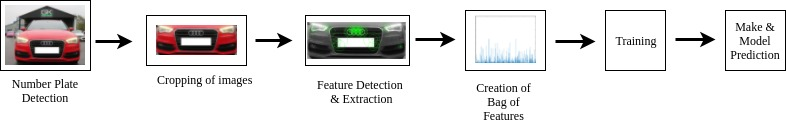
\includegraphics[scale=0.5]{VMMR.jpg}
  \caption{High level block diagram} \label{fig:blockdiagram} 
\end{figure}

The following sub-sections discuss the function of each block in the block diagram.

\subsubsection{Loaded images}
The first module of the system represents all the images that are loaded from the database. A datastore was created to hold the images within the subdirectories so as to ensure that all the image data is held centrally for easy access during the implementation phase. 

\subsubsection{Feature Detection}
It is at this stage that features or key points are detected within the image using a feature detector algorithm. These features include, edges, lines, blobs, corner points etc. The number of features detected depends on the input parameters passed to the feature detection algorithm. 

\subsubsection{Feature Extraction}
This is where the features or key points are extracted from the images based on the features detected by the feature detection algorithm. The feature extraction algorithm produces a feature vector containing the extracted features from a local bounding box within the image. 

\subsubsection{Creation of Bag of Features}
The bag of SURF features is created within this module after the features have been extracted by the feature extraction algorithm. K-means clustering is used to create a visual word vocabulary from the feature vectors obtained from the previous module.

\subsubsection{Training}
This is where a classifier, in this case, a support vector machine (SVM) is trained using the bag of SURF features and the corresponding labels. 

\subsubsection{Prediction of classes (Testing)}
Within this module, trained SVM attempts to predict the make and model of a car from an image within the validation or test set.

\subsubsection{Results}
This is where the predictions made by the support vector machine is evaluated against the actual outcome. 

\subsection{System Design}

\subsubsection{Loading the images}
The frontal view of various makes and models were captured and stored in the database. The images were placed into subdirectories according to the name of the make and model of each car. These images were preprocessed before they were loaded into the system. This was done in order to ensure that the program runs quicker and is less expensive computationally than preprocessing the images at run time. The preprocessing tasks that were carried out were cropping all images to obtain the frontal view of the car. Moreover, the image datastore was split into two sets that is, a training set and a validation set. Each subdirectory had a total of 25 images, therefore, it was decided to use 20 images for training and 5 images for testing. Hence 500 images were used for training and 125 images were used for testing. 

\subsubsection{Detection of SURF features} 
The bag of features approach was be used along with Speeded Up Robust Features (SURF) to create a bag of SURF features. Local SURF features were selected using the grid approach. 

\subsubsection{Extraction of SURF features}
The SURF features were extracted using an 8 by 8 patch and a bounding box which used the following coordinates [32 64 96 128].

\subsubsection{Creation of Bag of Features}
The bag of features was created from the extracted SURF features. After extraction, 80 percent of the strongest features also referred to as codewords were retained and the rest of the features are discarded. The number of features were then balanced across all categories in order to improve the efficiency of the k-means clustering (MathWorks, 2017). To balance the features, the algorithm locates the image which had the least amount of features obtained from a category and then selects the strongest amount of features from all categories based on this amount, therefore, the strongest amount of features selected throughout the images are the same. K-means clustering is used to generate a visual vocabulary of 5000 words, hence a total of 5000 clusters are created using the features.

\subsubsection{Training the classifier}
As stated earlier, a total of 500 images was used to train the image classifier. Before the training process begins, each of the training images are encoded to produce feature vectors for each category. These encoded images are then fed to the image classifier for training. As part of the training to evaluate whether training has been effective, the classifier is tested using the same training data. 

\subsubsection{Testing the classifier}
The classifier was tested using the test dataset created when the images were loaded. After predicting the make and models of the car, a confusion matrix is used to assess the performance of the classifier. Since there are 25 categories, this confusion matrix is a 25 by 25 matrix containing values which are used to determine the accuracy of the classifier. 

\newpage 
\section{ Experiments and Results }
This section discusses the experiments that were carried out on the proposed VMMR system including the results obtained from the experiments and proves the effectiveness of the classifier in recognising the makes and models of vehicles. 

\subsection{Experimental Design}
The experiments were carried out on a database of 650 images of vehicles grouped into 25 categories. Each category contained a total of 25 different images belonging to the same make and model.

The first experiment that was carried out was testing the performance of the classifier against the test set created at the start when the database was split into 2 sets (i.e. training set and test set).

The second experiment that was carried out made use of only 10 images in each category, therefore, 7 images were used for training and 3 images were used for testing. The purpose of this experiment was to compare the accuracy obtained from using only 7 images to the accuracy obtained when using a larger dataset that is, 20 images for training and 5 images for testing.  

The next experiment that was performed was to determine which feature detector and descriptor gave the best accuracy. The feature detectors/descriptors used were SURF and KAZE. Initially, the SURF features were detected and extracted from both the training images and the test images. The feature vectors were stored in separate matrices and passed to the SVM for both training and testing. A similar approach was taken with KAZE features. The use of SIFT for this project was considered however it was not used. The reason for this will be explained in the analysis section.

Since the bag of features approach was used in the implementation of the system, another experiment that was performed was to determine the effect of the visual vocabulary size on the accuracy of the classifier. The initial visual vocabulary size used was 500 words. This was increased to 1500, 3000 and 5000 respectively. Furthermore, the effects of changing certain parameters such as the point selection method and step size were also explored. This was to find the most effective parameter combination which provides a high level of accuracy with relatively low computational cost.

The final experiment that was carried out was to determine the performance of the trained support vector machine classifier on a new set of images. This new dataset was composed of 2 images for 10 makes and models that the classifier has been trained to recognise. The predict method of the classifier was used to determine which category the make and model the car belongs to. 


\subsection{ Results from experiments }

The confusion matrix in Figure 2 shows an analysis of the performance of the support vector machine classifier on the test dataset. 

\begin{figure}[!htb] 
  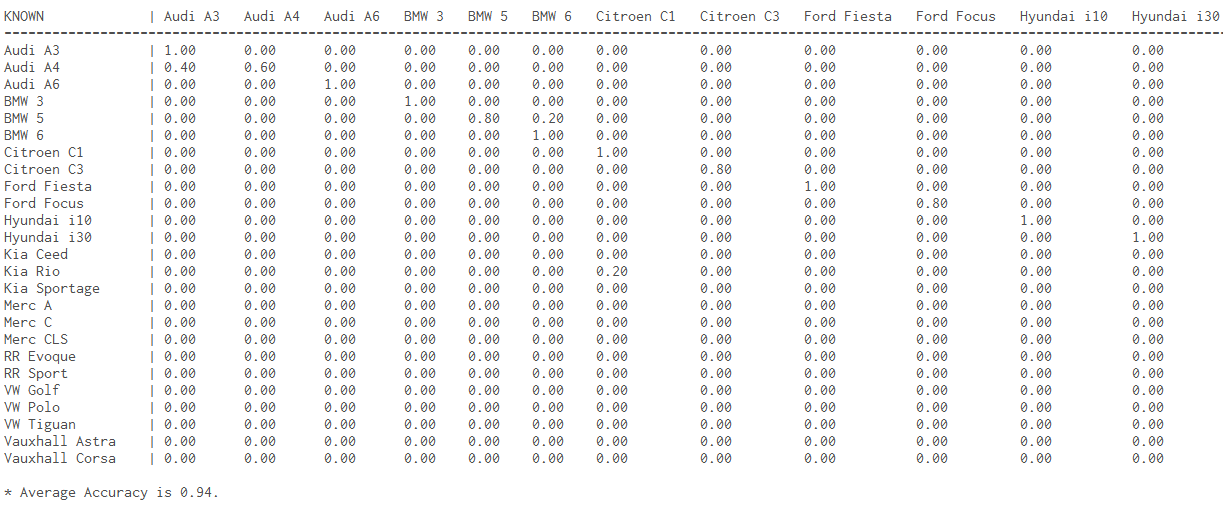
\includegraphics[scale=0.4]{confmatrix.png}
  \begin{center}
  	\caption{Confusion Matrix showing performance of classifier on test data set.}
  \end{center} 
  \label{fig:confmatrix} 
\end{figure}

After totalling the values on the diagonal, the accuracy value obtained was 94 percent. Based on this value, it can be concluded that the classifier performed very well overall in the recognition of the make and models of the various vehicles, nonetheless, it struggled to classify Audi A4 properly as only 60 percent of the images were recognised as Audi A4's. The other 40 percent of the Audi A4 images matched with Audi A3. Furthermore, It was hypothesised that using a larger dataset will yield better results. This hypothesis was proven to be true as using a larger dataset did increase the accuracy of the classifier. The accuracy improved from 30 percent to approximately 50 percent. 

Although SIFT is a very good detector/descriptor and is very feasible for this application, SIFT is very slow as compared to the other feature descriptors. According to the results obtained by Işik \& Özkan (2014), the computational time much greater (approximately 6.0 milliseconds) as compared with SURF (approximately 1.1 milliseconds). However, these figures may vary depending on the computer being used. Furthermore, although SURF was very quick the results obtained initially were appalling (30 percent). However, the results improved significantly when a feature vector size of 128 was used instead of 64 (50 percent). Despite the fact that KAZE was slower in terms of computational time, it produces better results than SURF given the same parameters. When KAZE features were used, the accuracy of the classifier went up to approximately 62 percent. These figures are presented in table 1 below. 

\begin{table}[!htb]
 \centering
 \textbf{\caption{Accuracy of descriptors using same paramters}}
 \begin{tabular}{|c|c|c|c|}
 \hline
  Detector/Descriptor & Metric Threshold & Feature Size & Accuracy (\%)\\
  \hline
  SURF & 2000 & 128 & 30 \\
  \hline 
  KAZE & 2000 & 128 & 62 \\
  \hline
 \end{tabular}
  
\end{table}

For the visual vocabulary size experiment, it was assumed that a larger vocabulary size would yield better results. This was proven to be true because, with a visual vocabulary size of 500 the accuracy of the classifier was found to be 80 percent. With a visual vocabulary size of 1500 words, the accuracy was found to be 84 percent. Furthermore, at 3000 words, accuracy of the classifier was found to be 85 percent. The best result was obtained when a vocabulary size of 5000 words were used (90 percent). 

\begin{table}[!htb]
 \centering
 \textbf{\caption{Accuracy of classifier using 80\% of strongest features}}
 \begin{tabular}{|c|c|c|c|}
 \hline
  Visual Vocabulary Size & Strongest Features (\%) & Accuracy (\%)\\
  \hline
   500 & 80 & 80 \\
  \hline 
   1500 & 80 & 84 \\
  \hline
   3000 & 80 & 85 \\
  \hline
   5000 & 80 & 90 \\
  \hline 
 \end{tabular}
\end{table}

The results varied slightly when the number of strongest features selected was increased from 80 percent to 100 percent. For a vocabulary size of 500, the accuracy of the classifier increased from 80 to 84 percent. For a vocabulary size of 1500 the accuracy increased from 84 percent to 90 percent. Similary for a vocabulary size of 3000 words, the accuracy increased from 85 percent to 89 percent. Additionally, for a vocabulary size of 5000, the accuracy improved to 93 percent. 

\begin{table}[!htb]
 \centering
 \textbf{\caption{Accuracy of classifier using 100\% of strongest features}}
 \begin{tabular}{|c|c|c|c|}
 \hline
  Visual Vocabulary Size & Strongest Features (\%) & Accuracy (\%)\\
  \hline
   500 & 100 & 84 \\
  \hline 
   1500 & 100 & 90 \\
  \hline
   3000 & 100 & 89 \\
  \hline
   5000 & 100 & 94 \\
  \hline 
 \end{tabular}
\end{table}

For the final experiment, the the classifier was able to predict each category correctly except for one category. The results are seen in table below: 

\begin{table}[!htb]
 \centering
 \textbf{\caption{Performance of classifier on new dataset}}
 \begin{tabular}{|c|c|c|c|}
 \hline
  Make \& Model & Accuracy (\%)\\
  \hline
   Audi A4 & 0 \\
  \hline 
   BMW 3 & 100 \\
  \hline
   Citroen & 100 \\
  \hline
   Ford Fiesta & 100 \\
  \hline 
   Hyundai i10 & 100 \\
   \hline 
   Kia Sportage & 100 \\
   \hline
   Mercedes-Benz C & 100 \\
   \hline
   Range Rover Sport & 100 \\
   \hline
   Vauxhaul Astra & 100 \\
   \hline
   VW Golf & 100 \\
   \hline
 \end{tabular}
\end{table}

Audi A4 was classified as Audi A3 rather than Audi A4.

\subsection{ Analysis of the results} 

From the first experiment, although the classifier manages to recognise almost all of the individual makes and models of the vehicles with 100 percent accuracy, it struggles with some of the vehicles especially Audi A4 as seen in Table 4 and in Figure 2. The reason for this is that, Audi A4 and Audi A3 look very similar in appearance, however they possess subtle differences. Examining this, it can be concluded that, some of the features detected in Audi A4 match with the features detected in Audi A3, hence, the same visual words may be used to describe these two vehicles. 

From the results obtained from the second experiment, it can be seen that the amount of data used for training and the accuracy of the classifier are directly proportional it can be concluded that, a larger dataset does improve the accuracy of the classifier. This is because, more images are being used for training and hence, the classifier becomes more accurate when predicting the make and models of the vehicles. Moreover, using a small amount of images will result in a poorly trained classifier as seen in the results above. In the second experiment, the KAZE and SURF feature detectors/descriptors performed poorly as compared with the bag of features approach. An explanation for this poor performance could be the manner in which the features were reduced. The feature extraction algorithms for these descriptors produced a set of feature vectors in the form of an M by 64 or M by 128 matrix for each image, depending on the size of the feature set specified. The error was introduced where the features in the feature matrices were summed up to produce a 1 by 64 or 1 by 128 feature vector for each image. This meant that all the features within the matrix were combined into form a row vector and this may have affected the performance of the classifier.

Similar to the first experiment, a relationship can be seen between the visual vocabulary size and the accuracy of the classifier, that is, the accuracy of the classifier improves with an increase in the vocabulary size. This is because with a larger vocabulary size, there are more visual words used to encode an image into a feature vector. Also, a likewise relationship exists between the number of strongest features selected and the accuracy obtained by the classifier. This is due to the fact that using more of the strongest features results in more feature descriptors being available for clustering and for the creation of visual words. 

\subsection{Conclusion}
\newpage
\section{Reference List} 

Cho,T.,S. (2010). \textit{Motion blur removal from photographs.} Submitted to the Department of Electrical Engineering and Computer Science in partial fulfilment of the requirements for the degree of Doctor of Philosophy in Electrical Engineering and Computer Science. Cambridge Massachusetts: Massachusetts Institute of Technology.
 
Freeman, W., J., T., Jones, T., R.,  Pasztor, E., C. (2002). Example-based super-resolution. \textit{IEEE Computer Graphics and Applications}, [Online] 22(2), pp.56-65. Available from: \url{http://ieeexplore.ieee.org/document/988747/} [Accessed 6 Jan. 2018].

Fisher, R., Perkins, S., Walker, A., Wolfart, E. (2003). \textit{Contrast Stretching}. [Online]. Available from: \url{https://homepages.inf.ed.ac.uk/rbf/HIPR2/stretch.htm} [Accessed 7th January 2018].

Gonzalez, C., R., Woods, E., R. (2008). \textit{Digital Image Processing.} Upper Saddle River New Jersey: Pearson.

Gribbon, K. T., Johnston, C. T., and Bailey, D.
G. \textit{A Real-time FPGA Implementation of a
Lens Distortion Correction Algorithm with
Bilinear Interpolation.} Proceedings of the
Image and Vision Computing New Zealand
Conference 2003, Massey University,
Palmerston North, New Zealand, Nov. 2003. pp. 408-413,

Hirsch, M., Schuler, C., Harmeling, S. and Scholkopf, B. (2011). Fast removal of non-uniform camera shake. 2011 International Conference on Computer Vision. [online] Available from: \url{http://ieeexplore.ieee.org/document/6126276/} [Accessed 5 Jan. 2018].

Işik, S., Özkan, K. (2014). A Comparative Evaluation of Well-known Feature Detectors and Descriptors. \textit{International Journal of Applied Mathematics, Electronics and Computers} [Online] 3(1), pp.1–6. Available from: \url{https://www.atscience.org/IJAMEC/article/download/135/83} [Accessed 10th January 2018].  

Kaur, S. (2015). Noise Types and Various Removal Techniques. \textit{International Journal of Advanced Research in Electronics and Communication Engineering (IJARECE). 4(2).} [Online] p.226-229. Available from \url{http://citeseerx.ist.psu.edu/viewdoc/download?doi=10.1.1.683.6783&rep=rep1&type=pdf
} [Accessed 5th January 2018].

MathWorks (2017). \textit{Image Category Classification Using Bag of Features}. [Online]. Available from: \url{https://uk.mathworks.com/help/vision/examples/image-category-classification-using-bag-of-features.html} [Accessed: 8th January 2018].

Patel, J., Shah, A., Patel, H. (2015). Skew Angle Detection and Correction using Radon Transform. \textit{International Journal of Electronics, Electrical and Computational System.} [Online] Volume 4 (May) Available from: \url{http://academicscience.co.in/admin/resources/project/paper/f201505101431314896.pdf}. [Accessed: 2nd January 2018].

Szeliski, R. (2010). \textit{Computer Vision: Algorithms and Applications.} New York: Springer.

Weng, C., C. Homer, C. Fuh, C., S. A Novel Automatic White Balance Method For Digital Still Cameras. 2005 \textit{IEEE International Symposium on Circuits and Systems.} [Online] Available from: \url{http://ieeexplore.ieee.org/abstract/document/1465458/} [Accessed 4 Jan. 2018].


\end{document}
